\chapter{Efficient Markets}

These notes follow Robert J. Shiller's lecture on efficient markets in \emph{Financial Markets}, curated by LazyingArt LLC. The lecture does not begin with a settled doctrine. It begins with a provocation. Efficient markets, Shiller says, is a half-truth. If prices already absorb public information, and if the market therefore ought to beat any one of us, what are we to do with David Swensen's long record at Yale? The lecture answers this by moving in a deliberate sequence: first through the weakness of simple performance statistics, then through the history of the efficient-markets idea, then through technical analysis as a rival way of reading prices, and finally through the random-walk and mean-reverting models that give the theory its mathematical spine.

\section{Opening paradox: efficient markets and David Swensen}

Shiller begins with the strongest classroom form of the hypothesis. Markets incorporate public information. Therefore we should not expect to outsmart the market by trading on what is already known. In the lecture's deliberately blunt slogan, the market knows more than we do, and if we think we can beat it, the market will usually win.

\begin{definition}
In the working sense of this lecture, the efficient-markets hypothesis says that publicly available information is incorporated into market prices so rapidly that one should not expect systematic excess profits from trading on that information after it has become public.
\end{definition}

That is already a sweeping proposition. But the lecture does not leave it in the abstract. Shiller brings in David Swensen, whose investment record at Yale had just been discussed in the previous class. Swensen is presented as someone who seems to have beaten the market over a very long period beginning in 1985, and with visible institutional consequences. Yale's financial strength supported policies such as wide need-blind access. Thus the opening problem is not merely statistical. It is institutional, human, and concrete.

\subsection{Question \& Answer}

If Swensen appears to beat the market for decades, is that skill, luck, or a problem with the theory?

Shiller refuses to settle the question with a slogan. A defender of efficient markets can always say that if millions of managers try, one of them will look brilliant by luck alone. But the reply comes quickly: twenty-five years is a long time to wave away with a one-line appeal to luck. At the same time, raw return alone cannot decide the matter. We must ask what risks were taken, how those risks were measured, and in what kinds of markets the manager chose to compete. That is why the lecture turns almost immediately to the Sharpe ratio.

\section{Sharpe ratios, hidden risk, and the temptation to game the statistics}

The bridge into the mathematics comes from a leftover question from Swensen's appearance. Why, if Yale's portfolio had done so well, did nobody talk about the Sharpe ratio? Shiller says he caught himself praising Yale's return without correcting for risk. That self-correction matters, because a high return by itself proves very little. Any expected return can be raised by taking more risk. That was already one of the lessons of the efficient frontier and the tangency line earlier in the course.

In the lecture's loose but serviceable form, we may write the Sharpe ratio as
\begin{equation}
S \approx \frac{E[R_p - R_b]}{\sigma(R_p)},
\end{equation}
where \(R_p\) is portfolio return and \(R_b\) is a benchmark return. In Shiller's spoken exposition the benchmark is ``the market,'' so we keep the symbol \(R_b\) only as a cautious notation choice.

The ingredients being summarized are the mean and standard deviation of return:
\begin{equation}
\mu_R = E[R], \qquad \sigma_R = \operatorname{SD}(R).
\end{equation}
A high excess return accompanied by a high standard deviation is not evidence of exceptional skill; it may merely be the compensation for taking exceptional risk.

Swensen's reply, as Shiller reconstructs it, is that for a broad portfolio full of illiquid assets the denominator may not be measurable in a clean way. Private equity is not continuously traded. Real estate may sit for years with only appraisals rather than repeated market transactions. Appraisal-based series smooth observed returns. In that case \(\sigma(R_p)\) can be artificially low before any deliberate manipulation has even begun.

\begin{figure}
\centering

\includegraphics[width=0.74\textwidth]{lecture_07_figure_02.png}
\caption{Bell-curve sketch for the return distribution. The frame supports a generic probability picture over a horizontal return axis, but not a fully labeled statistical graph.}
\end{figure}

Shiller then makes the argument harsher. Suppose a manager knows that the world will judge him by his Sharpe ratio. Suppose, further, that he has no ethical concern except to look good for a few years, gather assets, and walk away rich. The question becomes: what portfolio design makes the ratio look best, even if the underlying investment is rotten?

The answer, drawn from a paper by William Goetzmann and coauthors, is to reshape the tails. One begins with a bell-shaped return distribution. The mean and standard deviation of that distribution are what the Sharpe ratio sees. But the manager can alter the distribution itself. He can sell off the upper tail, giving away rare large gains in exchange for money now, and at the same time deepen the lower tail, so that rare bad outcomes become much worse. Most of the time nothing dramatic happens. The middle of the distribution looks calm. The portfolio records steady gains. The statistic looks beautiful. What has improved is not the investment. What has improved is the disguise.

\subsection{Question \& Answer}

How can a portfolio show a high Sharpe ratio while hiding catastrophic risk?

Because the Sharpe ratio only summarizes the realized sample. If the catastrophic left tail has not yet occurred, the reported mean and standard deviation can look entirely respectable. A manager who has clipped away rare upside and loaded rare downside receives income now, looks smooth for a while, and postpones the disaster to a future date. The true risk has not vanished. It has merely been pushed into rare states of the world that the sample has not yet visited.

Shiller's option language is informal, but the mechanism is clear. One may write away upside on the upper tail and otherwise create extra downside exposure through option positions. The point is not to produce a perfectly specified derivatives strategy on the board. The point is to understand how a statistic based on mean and standard deviation can be gamed by changing the unseen architecture of the tails.

\begin{figure}
\centering
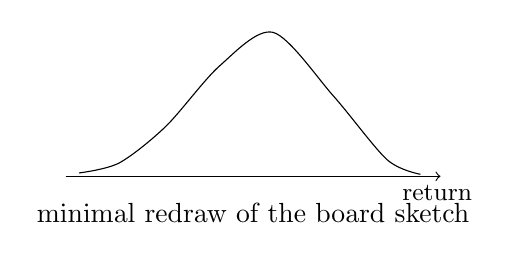
\begin{tikzpicture}[scale=0.85]
\draw[->] (0,0) -- (5.6,0);
\draw[smooth] plot coordinates {(0.2,0.05) (0.8,0.20) (1.5,0.75) (2.3,1.65) (3.1,2.15) (4.0,1.20) (4.8,0.25) (5.3,0.03)};
\node at (2.8,-0.55) {minimal redraw of the board sketch};
\node at (5.55,-0.25) {\small return};
\end{tikzpicture}
\hspace{1cm}
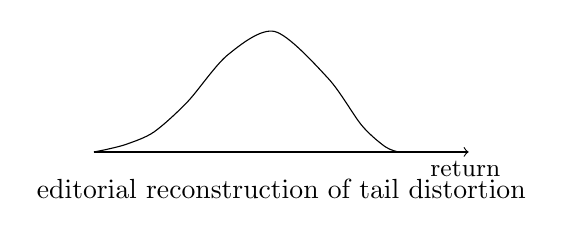
\begin{tikzpicture}[scale=0.85]
\draw[->] (0,0) -- (5.6,0);
\draw[smooth] plot coordinates {(0.0,0.00) (0.2,0.04) (0.5,0.12) (0.9,0.30) (1.4,0.75) (2.0,1.45) (2.7,1.80) (3.5,1.10) (4.0,0.40) (4.35,0.08) (4.55,0.00)};
\node at (2.8,-0.55) {editorial reconstruction of tail distortion};
\node at (5.55,-0.25) {\small return};
\end{tikzpicture}
\caption{Left: a cautious redraw of the bell-shaped return distribution visible on the board. Right: an editorial reconstruction of the lecture's verbal mechanism, with clipped upside and a heavier downside tail. The asymmetry on the right is transcript-based exposition, not a literal board redraw.}
\end{figure}

\section{Integral Investment Management, disclosure, and the moral of the Swensen recap}

At once Shiller says that this is not merely a blackboard trick. He points to Integral Investment Management, a hedge fund that used an options strategy of roughly this character. Investors poured money into it. Most notably, the Art Institute of Chicago put about \$43 million into the fund and related vehicles. When markets fell sharply in 2001, the strategy imploded and the Art Institute lost almost all of that investment.

The fund had looked extraordinary. That was the trap. A very high Sharpe ratio was mistaken for evidence of unusually good investing when in fact it was evidence that the measured statistics were concealing the true structure of the risk.

Shiller then sharpens the point further. The explicit derivatives trick is in one sense too obvious. Any experienced professional, once the strategy is laid bare, should recognize it. But the same logic can be implemented more subtly. One can simply buy firms or assets with large left tails: securities that carry a small probability of very large losses. For a while the returns look strong and the volatility looks low. Later the fund blows up. The lecture briefly gestures toward political tail risk of that kind, but the general lesson is sufficient: the market can hide bombs inside apparently ordinary securities.

This prepares the legal and moral turn. As Shiller states it, the law does not permit a manager to rely on boilerplate alone. If there is relevant information that would make the published statistics misleading, the manager must actively disclose it and make the client understand it. A generic sentence saying that past returns do not guarantee future results is not enough if the real issue is a specific embedded tail exposure.

The deeper moral returns us to Swensen. The substance of Swensen's achievement, Shiller suggests, is not mastery of a performance ratio. It has something to do with character, integrity, and the real objectives of the institution he serves. Statistics matter, but they do not tell the whole story. In real financial life, people judge not only numbers but persons and purposes. Only after this detour does Shiller say, in effect, that he wants now to go more directly into the lecture proper on efficient markets.

\section{Before the phrase: Gibson, Reuters, and Conant}

The lecture now resets historically. Shiller wants to reconstruct the intuition of efficient markets before the phrase itself became standard. The first clear statement he can find is George Gibson in 1889. Once shares are known in an open market, Gibson says, the value they acquire there may be taken as the judgment of the best intelligence concerning them.

This is already the core efficient-markets picture. The market is a voting mechanism, but not in the casual sense of polling opinions. If we think a share is undervalued, we buy. If we think it is overvalued, we sell. The better informed traders have stronger incentives to act and, if they succeed repeatedly, more capital with which to act. Price is therefore not the average thought of the public. It is a pressure point where the strongest and best-informed views are forced into action.

Just as important is the speed of information. Gibson writes in an electric age. In 1889 that means telegraphy, ticker machines, and rapid dissemination of quotes. The market is efficient, if it is efficient, not because wisdom falls from the sky, but because there is a relentless incentive to collect and transmit information faster than one's rivals.

\begin{figure}
\centering

\includegraphics[width=0.78\textwidth]{lecture_07_figure_03.png}
\caption{Gibson, Reuters, and Conant on the board. The arrangement is historically suggestive, but the frame should be read as board evidence rather than as a formal timeline.}
\end{figure}

Reuters gives this intuition its institutional form. Before the telegraph became dominant, Reuters used carrier pigeons to move financial information between cities. What sounds quaint is, economically, perfectly modern. If news can be moved even a little faster, money can be made. That is why information transmission becomes an industry. The pigeons are an early version of the same race that later uses telegraph wires, ticker machines, beepers, and electronic terminals.

Shiller makes the same point with a contemporary example. A firm announces a successful new drug. Analysts hear the news immediately. Within seconds and minutes they are on the telephone to specialists, revising estimates and trading before the rest of the public has even begun to process the announcement. Prices jump, overshoot, correct, and settle. By the next morning, when a newspaper reader decides he may want to buy the stock, the market is far ahead of him. This is the part of efficient markets that Shiller clearly wants us to keep. Public information becomes old information with astonishing speed.

This also begins to answer the Swensen puzzle. Shiller connects the point back to the prior lecture. In broad public markets such as bonds and large equities, even top-quartile managers may have little room to outdistance everyone else. But in unusual asset classes such as private equity or certain absolute-return strategies, public information is thinner and the market less crowded. Part of Swensen's achievement, then, may lie in choosing where the game is easier to play.

Conant, writing in 1904, gives the next major statement. He begins by rejecting the notion that stock-market speculation is merely gambling. That cannot be the whole truth, because the stock market is a central institution of the modern economy. If the stock exchanges of the world were closed, people would lose their public signals of value. Capital allocation would become blind. Economic calculation itself would be impaired.

\subsection{Question \& Answer}

Why is a stock market a central economic institution rather than just an organized gambling hall?

Because market prices do real social work. They summarize information, permit comparison, and help move capital from one use to another. Conant's point is not that gambling motives disappear in finance. It is that the market's deeper function is price discovery. Without quoted prices, investment decisions lose an indispensable guide. That is why a modern economy cannot simply dismiss speculation as morally noisy clutter. It is entangled with valuation itself.

\section{From doctrine to revision: Roberts, Fama, CRSP, and the softening of orthodoxy}

Only later does the phrase itself become standard. Shiller credits Harry Roberts at the University of Chicago with using the label, and Eugene Fama with making the idea famous. By then the theory had acquired something it did not possess in Gibson's or Conant's time: a modern data infrastructure.

In 1960 the Ford Foundation funded a large effort at Chicago to assemble reliable stock-price histories back to 1926, correcting for stock splits, dividends, and other details that had never been systematically organized. This became the Center for Research in Security Prices, now usually abbreviated CRSP. The famous tape was important not because tape is glamorous, but because finance could suddenly work with an organized universe of data rather than scraps from newspapers.

That changed the rhetoric of the theory. Once the data were assembled, the efficient-markets hypothesis could be tested on a scale that felt authoritative. By the end of the decade there were thousands of articles using the CRSP database. Fama's 1969 review article, \emph{Efficient Capital Markets}, gave the movement its canonical survey. His conclusion was not that every result favored efficiency, but that the evidence pointed toward remarkably efficient markets. The profession heard something stronger still: perhaps the very idea of beating the market was mostly a delusion.

The 1970s were therefore the high point of the doctrine. The theory did not merely describe prices. It seemed to discredit a vast investment industry. Successful managers, on this view, must mostly have been lucky. Yet Shiller's point is historical as well as analytical: the orthodoxy later weakened without becoming useless.

He shows this by turning to textbooks. Earlier editions of major finance texts could still say, with remarkable confidence, that security prices reflect the true underlying value of assets. Later editions retreated. They admitted that prices sometimes become badly misaligned with what appear to be discounted future payoffs. That is not a minor qualification. It is a substantial softening.

Shiller reinforces the point with Jonah Lehrer's phrase ``the truth wears off.'' The suggestion is not that science is fake or that earlier work was worthless. It is that an intellectual movement can begin with real insight, gather prestige, overstate its scope, and then be cut back by later evidence. Shiller even entertains the possibility that early enthusiasm itself can bias a research literature, just as it can in medicine or other sciences. Efficient markets, then, should be treated neither as a revelation nor as a dead theory. It should be treated as a strong idea that was once allowed to harden too far.

\section{Technical analysis as the foil}

After this long historical buildup, Shiller turns to technical analysis. The placement matters. Technical analysis is not introduced as a joke. It is introduced as a serious alternative to the efficient-markets mindset. Instead of reading balance sheets, economic news, or institutional structure, the technician reads price charts and looks for patterns in the path of prices themselves.

Edwards and McGee are the canonical figures here, and McGee appears as a psychologically minded analyst. He is so committed to price-reading that he wants an interior office with no windows, free from the distractions of the outside world. That anecdote is more than colorful. It captures the chartist conviction that the pattern is in the price, and that the price already contains the real drama.

Shiller gives two classic examples. The first is the resistance level. When the Dow first approached 1000, technicians thought it might have difficulty crossing such a psychologically imposing threshold. The second is the head-and-shoulders pattern, in which a higher peak is flanked by two lower peaks and is supposed to herald a collapse. McGee regarded these patterns as expressions of crowd psychology. The market, on this view, has moods that are visible in its shapes.

\subsection{Question \& Answer}

Does technical analysis actually work, or does it only find patterns in noise?

Shiller's answer is deliberately balanced. It is too simple to call technical analysis pure bunk. The efficient-markets literature in its strongest phase often dismissed chart reading more completely than the evidence warranted. Shiller even recounts asking Burton Malkiel, after \emph{A Random Walk Down Wall Street} appeared, where the many cited studies disproving technical analysis actually were. He suspected that the dismissal had outrun the bibliography. Later work did find some element of truth in some classic chartist observations.

But the opposite exaggeration is just as false. Technical analysis is not a machine for easy money. At best it is a subtle art that may occasionally augment broader judgment. That is precisely why the lecture now needs a stronger benchmark. If we are to decide whether patterns are meaningful, we must first understand what sheer unstructured price motion looks like. That benchmark is the random walk.

\section{Random walk, AR(1), and the half-truth conclusion}

The logical transition is direct. If prices are informationally efficient, then day-to-day price changes should come only from news. But news, as news, is unforecastable. Therefore price changes should themselves be unforecastable. This is the intuition behind the random walk.

\begin{definition}
A random walk is a process \(\{X_t\}\) whose one-step change is an unforecastable mean-zero shock.
\end{definition}

In symbols,
\begin{align}
X_t &= X_{t-1} + \epsilon_t, \\
E[\epsilon_t] &= 0,
\end{align}
where \(\epsilon_t\) is the innovation term. For classroom convenience Shiller allows us to imagine that the shocks have some standard deviation \(\sigma_\epsilon\) and perhaps even a Gaussian distribution:
\begin{equation}
\epsilon_t \sim N(0,\sigma_\epsilon^2).
\end{equation}
He later warns us not to trust the Gaussian approximation too much, but it is the easiest starting point.

Historically, the image is Carl Pearson's drunk at the lamppost. The drunk has no directional plan. Asked for a forecast of his position after some time, we do not infer a trend away from the lamppost. We take the current position as the center of the forecast and let the uncertainty widen with time. That is already the random-walk picture.

\begin{proposition}
If the shocks \(\epsilon_t\) are independent with mean zero, then for the random walk
\begin{equation}
E[X_{t+n}\mid X_t] = X_t,
\end{equation}
and the forecast dispersion obeys the square-root rule:
\begin{equation}
\operatorname{Var}(X_{t+n}-X_t) = n\sigma_\epsilon^2,
\qquad
\operatorname{SD}(X_{t+n}-X_t) = \sqrt{n}\,\sigma_\epsilon.
\end{equation}
\end{proposition}

\begin{proof}
Iterating the one-step equation gives
\[
X_{t+n}-X_t = \epsilon_{t+1}+\epsilon_{t+2}+\cdots+\epsilon_{t+n}.
\]
Conditional on \(X_t\), each shock has mean zero, so
\[
E[X_{t+n}-X_t\mid X_t]=0,
\]
which yields \(E[X_{t+n}\mid X_t]=X_t\). If the shocks are independent, their variances add:
\[
\operatorname{Var}(X_{t+n}-X_t)=\sum_{j=1}^n \operatorname{Var}(\epsilon_{t+j})=n\sigma_\epsilon^2.
\]
Taking square roots gives the square-root rule.
\end{proof}

This is the point at which the lecture turns back against technical analysis. A random walk can produce striking local patterns by accident. In fact Shiller's simulation later finds shapes that look head-and-shoulders-like even though the process generating them contains no true chartist signal at all. That is why the random walk is such a powerful foil: it teaches us how easily the eye invents structure.

Shiller then contrasts the random walk with the process written on the board in the lecture's final mathematical section. The screenshot preserves the blackboard comparison itself, and the comparison is part of the pedagogy.

\begin{figure}
\centering

\includegraphics[width=0.88\textwidth]{lecture_07_figure_05.png}
\caption{AR(1) process versus random walk. The screenshot matters here because it preserves the lecture's board layout: Pearson and \emph{Nature} 1905 at left, the mean-reverting alternative in the center, and the random walk at right.}
\end{figure}

Cleaned up into note-quality notation, the board comparison is
\begin{align}
X_t &= 100 + \rho(X_{t-1}-100) + \epsilon_t,
\qquad -1<\rho<1, \\
X_t &= X_{t-1} + \epsilon_t.
\end{align}
The right-hand shock term in the screenshot is not perfectly legible and looks closer to \(E_t\), but the transcript supports the standard reconstruction \(\epsilon_t\). The first equation is the AR(1) alternative, centered at 100; the second is the random walk.

The point of the AR(1) is mean reversion. The anchor level 100 plays the role of Pearson's lamppost. If the process is above 100, it tends to stay above 100 for a while, but it is pulled partway back. If it is below 100, it is pushed partway upward.

\begin{proposition}
For the AR(1) process
\[
X_t = 100 + \rho(X_{t-1}-100) + \epsilon_t,
\]
if \(E[\epsilon_t\mid X_{t-1}]=0\), then
\begin{equation}
E[X_t-100\mid X_{t-1}] = \rho(X_{t-1}-100).
\end{equation}
Hence when \(0<\rho<1\), deviations from 100 shrink in conditional expectation.
\end{proposition}

\begin{proof}
Subtract 100 from both sides:
\[
X_t-100 = \rho(X_{t-1}-100)+\epsilon_t.
\]
Now take conditional expectation given \(X_{t-1}\):
\[
E[X_t-100\mid X_{t-1}] = \rho(X_{t-1}-100) + E[\epsilon_t\mid X_{t-1}]
= \rho(X_{t-1}-100).
\]
If \(0<\rho<1\), the deviation keeps its sign but becomes smaller in magnitude on average.
\end{proof}

\paragraph{Worked example.}
Shiller gives the concrete classroom case \(\rho=\tfrac12\). If the previous observation is \(X_{t-1}=120\), then
\begin{equation}
E[X_t\mid X_{t-1}=120] = 100 + \frac12(120-100) = 110.
\end{equation}
The process is still above 100, but only half as far above as before. That is mean reversion in the simplest possible form.

\subsection{Question \& Answer}

Why does \(\rho=1\) turn the AR(1) process into a random walk, and what changes when \(\rho\) is only slightly below 1?

The algebra is immediate:
\begin{align}
X_t &= 100 + \rho(X_{t-1}-100) + \epsilon_t, \\
\rho=1 \quad \Longrightarrow \quad
X_t &= 100 + (X_{t-1}-100) + \epsilon_t \\
&= X_{t-1} + \epsilon_t.
\end{align}
So at \(\rho=1\) the anchor disappears from the law of motion. The process is no longer being pulled back. It is exactly the random walk.

If \(\rho\) is only slightly below 1, however, mean reversion is present but extremely weak. This is where Shiller introduces the loose-elastic-band metaphor. The drunk is still tied to the lamppost, but by a very loose elastic. He may wander for a long time before being pulled back. That is why an AR(1) with \(\rho=0.99\) or \(0.98\) can look very much like a random walk over realistic horizons, even though strict long-run mean reversion still exists.

The simulation segment makes this visible, though it does so in a slightly improvised way. Shiller compares actual long stock-market history with artificial series generated from random numbers. The striking point is that the random walk often looks uncannily like real market history. It produces booms, slumps, and plausible-looking patterns, even when no meaningful pattern has been built into the process.

He then compares those simulations with an AR(1) process. If \(\rho\) is substantially below 1, the process hugs its trend too tightly. In such a world profitable rules would be too easy: buy when the price is below trend and sell when it is above, because reversion is too reliable. Shiller's judgment is that the actual stock market does not look like that strong-reversion world.

At the same time, he corrects himself during the spreadsheet demonstration. Some of the simulated paths include an upward deterministic term. A stylized way to write that is
\begin{equation}
X_t = X_{t-1} + c + \epsilon_t,
\end{equation}
rather than a pure zero-drift random walk. The exact bookkeeping of the spreadsheet is not the heart of the lecture. The real lesson is comparative. A random walk, even with a simple drift term, often resembles long stock-market history more closely than a low-\(\rho\) AR(1) with strong mean reversion.

There is, however, a final caveat. The Gaussian random walk misses something important. In the simulation, Shiller does not get anything like the crash after 1929. The reason is not mysterious. A normal shock distribution has no fat tails:
\begin{equation}
\epsilon_t \sim N(0,\sigma_\epsilon^2)
\qquad \text{rules out the crash frequency we actually care about.}
\end{equation}
So even the random-walk model that best captures the shape of long market history remains only an approximation.

That is the lecture's last turn. The random walk is illuminating, because it teaches us how hard it is to extract genuine signals from price charts and how quickly public information is absorbed. But it is not the whole story. If the world is more like an AR(1) with \(\rho\) very close to 1 than like a perfect random walk, then there may be long-horizon opportunities, though not easy short-run ones. In that sense efficient markets is neither nonsense nor gospel. It is, just as Shiller said at the start, a half-truth.

\section{Summary}

The lecture begins with Swensen and ends with stochastic processes, but the path between them is the point. We first learn why raw performance statistics are inadequate and why the Sharpe ratio itself can be manipulated when tail risk is hidden. We then step back into the history of the idea, from Gibson's market as aggregated intelligence, through Reuters and the economics of information speed, to Conant's defense of speculation as price discovery rather than mere gambling. Only then do we arrive at the Chicago codification of the doctrine, its later softening, the challenge posed by technical analysis, and the random-walk versus AR(1) comparison that gives the lecture its mathematical payoff.

The conclusion is balanced in exactly the way the opening promised. Public information is absorbed rapidly, so simple money machines are elusive. Yet prices are not so perfect that every deviation from value disappears instantly, nor so Gaussian that crash risk fits neatly inside normal shocks. Efficient markets is useful because it captures something real. It is limited because it captures only part of what real financial markets do.